\chapter{راهنمای استفاده از الگوی لاتک دانشگاه صنعتی امیرکبیر(پلی‌تکنیک تهران)}

\section{مقدمه}
حروف‌چینی پروژه کارشناسی، پایان‌نامه یا رساله یکی از موارد پرکاربرد استفاده از زی‌پرشین است. از طرفی، یک پروژه، پایان‌نامه یا رساله،  احتیاج به تنظیمات زیادی از نظر صفحه‌آرایی  دارد که ممکن است برای
یک کاربر مبتدی، مشکل باشد. به همین خاطر، برای راحتی کار کاربر، یک کلاس با نام 
\verb;AUTthesis;
 برای حروف‌چینی پروژه‌ها، پایان‌نامه‌ها و رساله‌های دانشگاه صنعتی امیرکبیر با استفاده از نرم‌افزار زی‌پرشین،  آماده شده است. این فایل به 
گونه‌ای طراحی شده است که کلیه خواسته‌های مورد نیاز  مدیریت تحصیلات تکمیلی دانشگاه صنعتی امیرکبیر را برآورده می‌کند و نیز، حروف‌چینی بسیاری
از قسمت‌های آن، به طور خودکار انجام می‌شود.

کلیه فایل‌های لازم برای حروف‌چینی با کلاس گفته شده، داخل پوشه‌ای به نام
\verb;AUTthesis;
  قرار داده شده است. توجه داشته باشید که برای استفاده از این کلاس باید فونت‌های
  \verb;Nazanin B;،
 \verb;PGaramond;
 و
  \verb;IranNastaliq;
    روی سیستم شما نصب شده باشد.
\section{این همه فایل؟!}\label{sec2}
از آنجایی که یک پایان‌نامه یا رساله، یک نوشته بلند محسوب می‌شود، لذا اگر همه تنظیمات و مطالب پایان‌نامه را داخل یک فایل قرار بدهیم، باعث شلوغی
و سردرگمی می‌شود. به همین خاطر، قسمت‌های مختلف پایان‌نامه یا رساله  داخل فایل‌های جداگانه قرار گرفته است. مثلاً تنظیمات پایه‌ای کلاس، داخل فایل
\verb;AUTthesis.cls;، 
تنظیمات قابل تغییر توسط کاربر، داخل 
\verb;commands.tex;،
قسمت مشخصات فارسی پایان‌نامه، داخل 
\verb;fa_title.tex;,
مطالب فصل اول، داخل 
\verb;chapter1;
و ... قرار داده شده است. نکته مهمی که در اینجا وجود دارد این است که از بین این  فایل‌ها، فقط فایل 
\verb;AUTthesis.tex;
قابل اجرا است. یعنی بعد از تغییر فایل‌های دیگر، برای دیدن نتیجه تغییرات، باید این فایل را اجرا کرد. بقیه فایل‌ها به این فایل، کمک می‌کنند تا بتوانیم خروجی کار را ببینیم. اگر به فایل 
\verb;AUTthesis.tex;
دقت کنید، متوجه می‌شوید که قسمت‌های مختلف پایان‌نامه، توسط دستورهایی مانند 
\verb;input;
و
\verb;include;
به فایل اصلی، یعنی 
\verb;AUTthesis.tex;
معرفی شده‌اند. بنابراین، فایلی که همیشه با آن سروکار داریم، فایل 
\verb;AUTthesis.tex;
است.
در این فایل، فرض شده است که پایان‌نامه یا رساله شما، از5 فصل و یک پیوست، تشکیل شده است. با این حال، اگر
  پایان‌نامه یا رساله شما، بیشتر از 5 فصل و یک پیوست است، باید خودتان فصل‌های بیشتر را به این فایل، اضافه کنید. این کار، بسیار ساده است. فرض کنید بخواهید یک فصل دیگر هم به پایان‌نامه، اضافه کنید. برای این کار، کافی است یک فایل با نام 
\verb;chapter6;
و با پسوند 
\verb;.tex;
بسازید و آن را داخل پوشه 
\verb;AUTthesis;
قرار دهید و سپس این فایل را با دستور 
\texttt{\textbackslash include\{chapter6\}}
داخل فایل
\verb;AUTthesis.tex;
و بعد از دستور
\texttt{\textbackslash include\{chapter6\}}
 قرار دهید.

\section{از کجا شروع کنم؟}
قبل از هر چیز، بدیهی است که باید یک توزیع تِک مناسب مانند 
\verb;Live TeX;
و یک ویرایش‌گر تِک مانند
\verb;Texmaker;
را روی سیستم خود نصب کنید.  نسخه بهینه شده 
\verb;Texmaker;
را می‌توانید  از سایت 
 \href{http://www.parsilatex.com}{پارسی‌لاتک}%
\LTRfootnote{\url{http://www.parsilatex.com}}
 و
\verb;Live TeX;
را هم می‌توانید از 
 \href{http://www.tug.org/texlive}{سایت رسمی آن}%
\LTRfootnote{\url{http://www.tug.org/texlive}}
 دانلود کنید.
 
در مرحله بعد، سعی کنید که  یک پشتیبان از پوشه 
\verb;AUTthesis;
 بگیرید و آن را در یک جایی از هارددیسک سیستم خود ذخیره کنید تا در صورت خراب کردن فایل‌هایی که در حال حاضر، با آن‌ها کار می‌کنید، همه چیز را از 
 دست ندهید.
 
 حال اگر نوشتن پایان‌نامه اولین تجربه شما از کار با لاتک است، توصیه می‌شود که یک‌بار به طور سرسری، کتاب «%
\href{http://www.tug.ctan.org/tex-archive/info/lshort/persian/lshort.pdf}{مقدمه‌ای نه چندان کوتاه بر
\lr{\LaTeXe}}\LTRfootnote{\url{http://www.tug.ctan.org/tex-archive/info/lshort/persian/lshort.pdf}}»
   ترجمه دکتر مهدی امیدعلی، عضو هیات علمی دانشگاه شاهد را مطالعه کنید. این کتاب، کتاب بسیار کاملی است که خیلی از نیازهای شما در ارتباط با حروف‌چینی را برطرف می‌کند.
 
 
بعد از موارد گفته شده، فایل 
\verb;AUTthesis.tex;
و
\verb;fa_title;
را باز کنید و مشخصات پایان‌نامه خود مثل نام، نام خانوادگی، عنوان پایان‌نامه و ... را جایگزین مشخصات موجود در فایل
\verb;fa_title;
 کنید. دقت داشته باشید که نیازی نیست 
نگران چینش این مشخصات در فایل پی‌دی‌اف خروجی باشید. فایل 
\verb;AUTthesis.cls;
همه این کارها را به طور خودکار برای شما انجام می‌دهد. در ضمن، موقع تغییر دادن دستورهای داخل فایل
\verb;fa_title;
 کاملاً دقت کنید. این دستورها، خیلی حساس هستند و ممکن است با یک تغییر کوچک، موقع اجرا، خطا بگیرید. برای دیدن خروجی کار، فایل 
\verb;fa_title;
 را 
\verb;Save;، 
(نه 
\verb;As Save;)
کنید و بعد به فایل 
\verb;AUTthesis.tex;
برگشته و آن را اجرا کنید. حال اگر می‌خواهید مشخصات انگلیسی پایان‌نامه را هم عوض کنید، فایل 
\verb;en_title;
را باز کنید و مشخصات داخل آن را تغییر دهید.%
\RTLfootnote{
برای نوشتن پروژه کارشناسی، نیازی به وارد کردن مشخصات انگلیسی پروژه نیست. بنابراین، این مشخصات، به طور خودکار،
نادیده گرفته می‌شود.
}
 در اینجا هم برای دیدن خروجی، باید این فایل را 
\verb;Save;
کرده و بعد به فایل 
\verb;AUTthesis.tex;
برگشته و آن را اجرا کرد.

برای راحتی بیشتر، 
فایل 
\verb;AUTthesis.cls;
طوری طراحی شده است که کافی است فقط  یک‌بار مشخصات پایان‌نامه  را وارد کنید. هر جای دیگر که لازم به درج این مشخصات باشد، این مشخصات به طور خودکار درج می‌شود. با این حال، اگر مایل بودید، می‌توانید تنظیمات موجود را تغییر دهید. توجه داشته باشید که اگر کاربر مبتدی هستید و یا با ساختار فایل‌های  
\verb;cls;
 آشنایی ندارید، به هیچ وجه به این فایل، یعنی فایل 
\verb;AUTthesis.cls;
دست نزنید.

نکته دیگری که باید به آن توجه کنید این است که در فایل 
\verb;AUTthesis.cls;،
سه گزینه به نام‌های
\verb;bsc;,
\verb;msc;
و
\verb;phd;
برای تایپ پروژه، پایان‌نامه و رساله،
طراحی شده است. بنابراین اگر قصد تایپ پروژه کارشناسی، پایان‌نامه یا رساله را دارید، 
 در فایل 
\verb;AUTthesis.tex;
باید به ترتیب از گزینه‌های
\verb;bsc;،
\verb;msc;
و
\verb;phd;
استفاده کنید. با انتخاب هر کدام از این گزینه‌ها، تنظیمات مربوط به آنها به طور خودکار، اعمل می‌شود.

\section{مطالب پایان‌نامه را چطور بنویسم؟}
\subsection{نوشتن فصل‌ها}
همان‌طور که در بخش 
\ref{sec2}
گفته شد، برای جلوگیری از شلوغی و سردرگمی کاربر در هنگام حروف‌چینی، قسمت‌های مختلف پایان‌نامه از جمله فصل‌ها، در فایل‌های جداگانه‌ای قرار داده شده‌اند. 
بنابراین، اگر می‌خواهید مثلاً مطالب فصل ۱ را تایپ کنید، باید فایل‌های 
\verb;AUTthesis.tex;
و
\verb;chapter1;
را باز کنید و محتویات داخل فایل 
\verb;chapter1;
را پاک کرده و مطالب خود را تایپ کنید. توجه کنید که همان‌طور که قبلاً هم گفته شد، تنها فایل قابل اجرا، فایل 
\verb;AUTthesis.tex;
است. لذا برای دیدن حاصل (خروجی) فایل خود، باید فایل  
\verb;chapter1;
را 
\verb;Save;
کرده و سپس فایل 
\verb;AUTthesis.tex;
را اجرا کنید. یک نکته بدیهی که در اینجا وجود دارد، این است که لازم نیست که فصل‌های پایان‌نامه را به ترتیب تایپ کنید. می‌توانید ابتدا مطالب فصل ۳ را تایپ کنید و سپس مطالب فصل ۱ را تایپ کنید.

نکته بسیار مهمی که در اینجا باید گفته شود این است که سیستم
\lr{\TeX},
محتویات یک فایل تِک را به ترتیب پردازش می‌کند. به عنوان مثال، اگه فایلی، دارای ۴ خط دستور باشد، ابتدا خط ۱، بعد خط ۲، بعد خط ۳ و در آخر، خط ۴ پردازش می‌شود. بنابراین، اگر مثلاً مشغول تایپ مطالب فصل ۳ هستید، بهتر است
که دو دستور
\verb~\chapter{مقدمه}
\section{مقدمه}

یادگیری ماشین\footnote{\lr{Machine Learning}} یک سیستم را قادر می‌سازد تا داده‌ها را بررسی کند و دانش را استنباط کند. الگوهای آموخته‌شده برای تجزیه و تحلیل داده‌های ناشناخته استفاده می‌شوند، به گونه‌ای که می‌توان آنها را گروه بندی کرد یا به گروه‌های شناخته شده آنها را تقسیم بندی کرد. تکنیک‌های اولیه یادگیری ماشین غیر قابل انعطاف بوده و قادر به تغییری در داده‌های آموزشی نیستند. پیشرفت‌های اخیر در یادگیری ماشین باعث شده این تکنیک‌ها در دنیای واقعی انعطاف پذیر و مقاوم باشند.
\\
موفقیت تکنیک‌های یادگیری ماشین تا حد زیادی به داده‌ها وابسته‌است. داده‌های عظیم در شبکه‌های امروزی وجود دارد که با شبکه‌های در حال ظهوری مانند اینترنت اشیا و میلیاردها دستگاه متصل به آن، رشد بیشتری خواهدکرد. به همین دلیل کاربرد یادگیری ماشین بیشتر خواهدشد که نه تنها الگوهای پنهان را شناسایی کند، بلکه می‌تواند برای یادگیری و درک فرایندهای تولید داده نیز به کار رود.
\\
علیرغم پیشرفت‌ها در یادگیری ماشین، عملیات و مدیریت شبکه همچنان دشوار است و خطاهای شبکه عمدتا به دلیل خطای انسانی شایع است. از طرفی الگوهای ثابت در یک شبکه ممکن است برای شبکه دیگری از همان نوع عملی نباشد. همچنین، شبکه به طور مداوم در حال تکامل است و پویایی‌ها مانع از استفاده از یک مجموعه ثابت از الگوهایی می‌شوند که به عملکرد و مدیریت شبکه کمک کند.
\\
پیشرفت‌های کلیدی در شبکه، از جمله قابلیت برنامه نویسی شبکه از طریق شبکه نرم افزاری\footnote{\lr{SDN}}، کاربرد یادگیری ماشین را در شبکه ارتقا می‌بخشد. یکی از موانع اصلی موفقیت در شبکه‌ این است که چه داده‌هایی می تواند از آن جمع شود و چه اقدامات کنترلی را می توان در دستگاه‌های شبکه انجام داد. توانایی برنامه‌ریزی شبکه با استفاده از شبکه نرم افزاری این موانع را برطرف می‌کند. استفاده از تکنیک‌های یادگیری ماشین برای چنین مشکلات متنوع و پیچیده‌ای در شبکه مفید است. این امر باعث می‌شود یادگیری ماشین در شبکه به یک زمینه تحقیقاتی جالب توجه تبدیل شود\cite{boutaba2018comprehensive}.

\newpage

پژوهش‌های متنوعی درباره یادگیری ماشین در شبکه وجود دارد، اما این پژوهش به دلیل جامع بودن تکنیک های یادگیری ماشین تحت پوشش و جنبه های مختلف شبکه صرف نظر از فن آوری شبکه متفاوت است. در این گزارش ابتدا در مورد انواع مختلف تکنیک های مبتنی بر یادگیری ماشین، ترکیبات اساسی و تکامل آنها بررسی می‌کنیم. سپس سیر تحول و کاربردهای مباحث زیر را به ترتیب خواهیم گفت.


\begin{enumerate}
    \item مهندسی ترافیک
    \begin{itemize}
        \item پیشبینی ترافیک
        \item طبقه‌بندی ترافیک
        \item مسیریابی ترافیک
    \end{itemize}
    
    
    \item کارایی و بهینه‌سازی
    \begin{itemize}
        \item کنترل ازدحام
        \item مدیریت کیفیت سرویس\footnote{\lr{QoS}} و تجربه\footnote{\lr{QoE}}
        \item مدیریت منابع و خطا
    \end{itemize}
    \item امنیت شبکه
    
\end{enumerate}


و در نهایت فرصت‌های تحقیقاتی موجود را اشاره می‌کنیم.
~
و
\verb~\chapter{یادگیری ماشین}
در سال 1959، آرتور ساموئل اصطلاح یادگیری ماشین را به عنوان زمینه‌ای که به کامپیوتر توانایی یادگیری بدون برنامه‌ریزی صریح را می‌دهد ابداع کرد،. چهار دسته گسترده از مسائل وجود دارد که می‌توان از یادگیری ماشین در آنها استفاده‌کرد:
\begin{enumerate}
    \item خوشه‌ بندی\LTRfootnote{\lr{Clustering}}:
    گروه بندی داده‌های مشابه باهم با افزایش فاصله بین گروه‌ها 
    \item طبقه ‌بندی\LTRfootnote{\lr{Classification}}: نگاشت مجموعه‌ای از داده‌های جدید به مجموعه‌ای با مقادیر گسسته 
    \item رگرسیون\LTRfootnote{\lr{Regression}}: نگاشت مجموعه‌ای از داده‌های جدید به مجموعه‌ای با مقادیر پیوسته
    \item استخراج قاعده\LTRfootnote{\lr{Rule Extraction}}: شناسایی روابط آماری در داده‌ها 
\end{enumerate}

روشی کلی برای ساختن راه حل‌های مبتنی بر یادگیری ماشین وجود دارد \cref{fig.1}. که در ادامه به بررسی مختصر هرکدام از اجزا می‌پردازیم.

\begin{figure}[!h]
\centering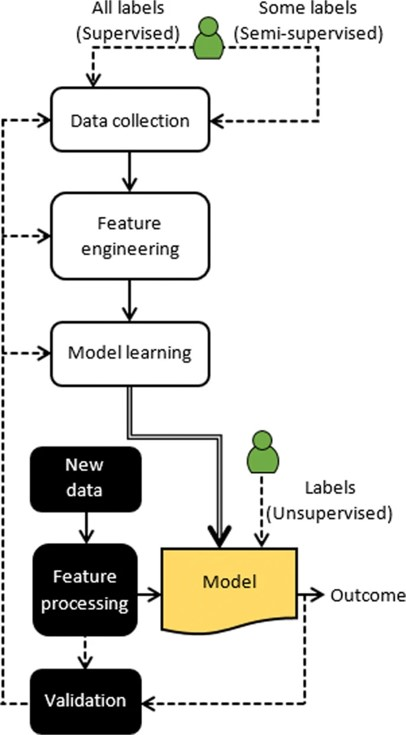
\includegraphics[scale=.8]{./figures/Solution}
\caption{اجزاء سازنده‌ی راه حل‌های مبتنی بر یادگیری ماشین}\label{fig.1}
\end{figure}

\newpage

\section{الگوهای یادگیری}

در یادگیری ماشین چهار الگوی یادگیری وجود دارد، این الگوها بر مراحل بعدی تأثیر می‌گذارند. هدف کلی این است که با توجه به برخی از مجموعه‌های داده نتیجه بگیریم. این الگوها برپایه‌ی دو روش فکری مولد  \LTRfootnote{\lr{Generative}}  و متمایزکننده \LTRfootnote{\lr{Discriminative}} هستند که ریشه در قانون بیز  \LTRfootnote{\lr{Bayes’ Theorem}} دارند:

\begin{equation}
    P(A|B) = \frac{P(B|A)*P(A)}{P(B)}
\end{equation}

%$$
%P(A|B) = \frac{P(B|A)*P(A)}{P(B)}
%$$
این چهار الگوی یادگیری عبارتند از:
\begin{itemize}
\item تحت نظارت\LTRfootnote{\lr{Supervised Learning}}: در حل مسائل طبقه‌بندی و رگرسیون کاربرد دارد و از مجموعه داده‌های برچسب‌دار برای مدل کردن استفاده می‌کنند.
\item نیمه نظارت\LTRfootnote{\lr{Semi-supervised Learning}}: اگر برچسب‌ها ناقص باشند از یادگیری نیمه نظارتی استفاده می‌شود.
\item بدون نظارت\LTRfootnote{\lr{Unsupervised Learning}}: اگر داده‌ها بی‌برچسب باشند از یادگیری بدون نظارت استفاده خواهد شد. از این روش بیشتر در مسائل خوشه بندی استفاده می‌شود.
\item تقویتی\LTRfootnote{\lr{Reinforcement Learning(RL)}}: یک فرایند تکراری مبتنی بر عامل است. عامل در محیط به کاوش می‌پردازد و درنهایت آن را بر اساس اعمالش تشویق و یا جریمه می‌کند. درواقع مجموعه داده‌ها شامل همین تشویق و جریمه‌ها می‌باشند. همچنین با دریافت بازخورد از محیط، کاوش‌های بعدی را تعیین می‌شود.
\end{itemize}



\newpage


\section{جمع‌آوری داده}

تکنیک‌های یادگیری ماشین برای ساخت یک مدل موثر یادگیری ماشین برای یک مشکل خاص، نیاز به داده دارند. جمع آوری داده‌ها یک مرحله مهم است، زیرا داده‌ها نه تنها از یک مسئله به مسئله دیگر بلکه در دوره‌های زمانی نیز باهم متفاوت هستند. به طور کلی جمع آوری داده در دو فاز انجام میشود:
\begin{itemize}
\item آفلاین: این امکان را به ما می‌دهد تا داده‌های مربوط به گذشته برای آموزش و تست مدل به کار روند.
\item آنلاین: این امکان را به ما می‌دهد تا داده‌های شبکه در زمان حال برای بازخورد و ورودی برای آموزش مجدد به کار روند.
\end{itemize}

یک منبع برای جمع آوری داده در هر دوفاز استفاده از ابزارهای نظارتی و اندازه گیری، در سطح شبکه است که میتواند به صورت‌های زیر باشد:

\begin{itemize}
\item نظارت فعال: ترافیک اندازه گیری را تزریق می‌کند، مانند بسته‌های پروب \LTRfootnote{\lr{Probe}} در شبکه و داده‌های مربوطه را از این ترافیک جمع آوری می‌کند.
\item نظارت غیرفعال: با مشاهده میزان واقعی ترافیک شبکه، داده‌ها را جمع آوری می‌کند.
\end{itemize}

نظارت فعال به دلیل مصرف پهنای باند از ترافیک تزریقی، هزینه اضافی را به دنبال دارد. در حالیکه، نظارت غیرفعال با هزینه دستگاه‌های اضافی که ترافیک شبکه را برای جمع آوری اطلاعات مربوطه تجزیه و تحلیل می‌کنند، این سربار را از بین می‌برد\cite{ boutaba2018comprehensive}.
\\
پس از جمع آوری داده‌ها، آنها به مجموعه‌های آموزش، اعتبار سنجی و آزمون تجزیه می‌شوند. مجموعه آموزش برای یافتن پارامترهای ایده آل، مجموعه اعتبار سنجی برای انتخاب معماری مناسب و مجموعه آزمون برای ارزیابی عملکرد بی‌طرفانه مدل انتخاب شده استفاده می‌شود. اینکه چه درصدی از داده‌ها را به کدام مجموعه اختصاص دهیم باید با توجه به کلاس‌های مورد علاقه صورت گیرد.
\newpage

\section{مهندسی ویژگی}



داده‌های خام جمع آوری شده ممکن است اضافی یا ناقص باشند. قبل از استفاده از داده‌ها برای یادگیری، باید مرحله قبل از پردازش را طی کرد. مرحله مهم دیگر قبل از یادگیری، یا آموزش یک مدل، استخراج ویژگی است.


مهندسی ویژگی یک جنبه حیاتی در یادگیری ماشین است که شامل انتخاب و استخراج ویژگی است. برای کاهش ابعاد در داده‌های حجیم و شناسایی ویژگی‌های متمایز که سربار محاسباتی را کاهش می‌دهد استفاده می‌شود. استخراج ویژگی‌ها معمولاً یک فرآیند محاسباتی فشرده است که با استفاده از تکنیک‌هایی مانند آنتروپی و تبدیل فوریه از ویژگی‌های موجود می‌توان ویژگی‌های جدیدی را به دست آورد\cite{ boutaba2018comprehensive}.


\section{ایجاد حقیقت عینی}


ایجاد حقیقت عینی درواقع دادن توصیف رسمی (به عنوان مثال برچسب) به کلاس‌های مورد علاقه است. حقیقت عینی دقت مدل‌های یادگیری ماشین را به همراه دارد. همچنین وابستگی متقابل بین داده‌های آموزشی یک کلاس مورد علاقه به کلاس دیگر وجود دارد که بر عملکرد مدل تأثیر می گذارد. عدم تعادل در تعداد داده‌های آموزش در بین کلاس ها، فرضیاتی را که بسیاری از تکنیک‌های یادگیری ماشین دارند، نقض میکند. بنابر این با استفاده از انواع روش‌های نمونه برداری باید تعادل را برقرار کرد\cite{ boutaba2018comprehensive}.



\section{شاخص‌های عملکرد و اعتبارسنجی مدل}

هنگامی که یک مدل یادگیری ماشین ساخته شد و حقیقت عینی مشخص شد، ارزیابی عملکرد مدل یادگیری ماشین که نتایج را توصیف، پیش بینی یا ارزیابی می‌کند، بسیار مهم است. همچنین، باید توجه کنیم که هیچ راهی برای تشخیص الگوریتم یادگیری به عنوان بهترین الگوریتم وجود ندارد و مقایسه میزان خطا در طیف وسیعی از برنامه‌ها عادلانه نیست. از معیارهای عملکرد می‌توان برای اندازه گیری جنبه‌های مختلف مدل مانند قابلیت اطمینان، استحکام، دقت و پیچیدگی استفاده کرد.

%\section{تکامل روش‌های یادگیری ماشین}

\newpage

\section{خلاصه}


در این فصل، روشي كلي براي ساختن راه حل هاي مبتني بر يادگيري ماشين را ارائه دادیم. در ابتدا، انواع الگوهای یادگیری تحت نظارت، نیمه نظارت، بدون نظارت و تقویتی را دیدیم. سپس مرحله جمع آوری داده ها وجود دارد که به صورت آفلاین و آنلاین انجام می‌شود. سپس به سراغ استخراج ویژگی‌ها رفتیم که برای جلوگیری از سربار محاسباتی مرحله‌ای مهم است. بعد از آن ایجاد حقیقت عینی را دیدیم که می‌بایست به نحوی انجام بشود که تعادل در تعداد داده‌های آموزش برقرار شود. و در مرحله آخر می‌بایست مدل تولید شده را مورد اعتبارسنجی و ارزیابی قرار داد.

~
را در فایل 
\verb~AUTthesis.tex~،
غیرفعال%
\RTLfootnote{
برای غیرفعال کردن یک دستور، کافی است پشت آن، یک علامت
\%
 بگذارید.
}
 کنید. زیرا در غیر این صورت، ابتدا مطالب فصل ۱ و ۲ پردازش شده (که به درد ما نمی‌خورد؛ چون ما می‌خواهیم خروجی فصل ۳ را ببینیم) و سپس مطالب فصل ۳ پردازش می‌شود و این کار باعث طولانی شدن زمان اجرا می‌شود. زیرا هر چقدر حجم فایل اجرا شده، بیشتر باشد، زمان بیشتری هم برای اجرای آن، صرف می‌شود.

\subsection{مراجع}
برای وارد کردن مراجع به فصل 2
مراجعه کنید.
\subsection{واژه‌نامه فارسی به انگلیسی و برعکس}
برای وارد کردن واژه‌نامه فارسی به انگلیسی و برعکس، بهتر است مانند روش بکار رفته در فایل‌های 
\verb;dicfa2en;
و
\verb;dicen2fa;
عمل کنید.

\section{اگر سوالی داشتم، از کی بپرسم؟}
برای پرسیدن سوال‌های خود در مورد حروف‌چینی با زی‌پرشین،  می‌توانید به
 \href{http://forum.parsilatex.com}{تالار گفتگوی پارسی‌لاتک}%
\LTRfootnote{\url{http://www.forum.parsilatex.com}}
مراجعه کنید. شما هم می‌توانید روزی به سوال‌های دیگران در این تالار، جواب بدهید.
